
\section{Application Evaluation}
\label{sec:apps}
Legion is a high-level runtime system that has been implemented on top
of our interface\cite{Legion12}.  
%The Legion runtime is distributed so 
%that there is an independent scheduler for each processor in the machine.  
The Legion programming model is built around the abstraction of 
{\em logical regions} which express locality and independence properties 
of data.  Computation in Legion is organized into a tree of tasks where 
each task must specify which logical regions will be accessed.
When executing a Legion task, the Legion runtime receives requests
to execute sub-tasks along with their region requirements.
This stream of tasks with region requirements is analogous to a stream
of instructions with register requirements that are executed by 
a hardware processor.  Hardware out-of-order processors are designed to
run ahead of the actual execution of a stream of instructions
to ensure that the processor's pipeline is fully utilized.  Similarly, on
every processor of a supercomputer there is an instance of the Legion runtime
that takes a stream of tasks with region requirements and asynchronously
runs ahead of the actual execution using a {\em software-out-of-order} (SOOP)
scheduler.  The details of the SOOP are beyond the scope of this paper
but are described in \cite{Legion12}.

The fully asynchronous design of the interface that we've proposed in
this paper is crucial to Legion's SOOP implementation.  Without a fully
asynchronous interface, the SOOP would have to periodically invoke
blocking operations that would cause processors to stall and severly
limit Legion's ability to run-ahead and keep the machine fully
occupied.  With a fully asynchronous interface the SOOP can run
far ahead of the actual execution, limited only by the physical resources
available in the machine, exactly like a hardware out-of-order processor.

In this section we demonstrate the performance properties of three
real-world applications that use the Legion runtime and consequently the heterogeneous
implementation of our interface to run on the Keeneland supercomputer.
The three applications that we characterize are all multi-phase
applications that require parallel computation, data exchange, and
synchronization between phases. 
\begin{itemize} \itemsep1pt \parskip0pt \parsep0pt
\item Circuit - 
\item Fluid -
\item AMR - 
\end{itemize}
In Section~\ref{subsec:eventlife} we show properties of events in
the Fluid application.  Section~\ref{subsec:lockmig} examines
the migration of locks in the Fluid application.  We give
a brief case study of reductions for the Circuit application
in Section~\ref{subsec:reduccase}.  Finally, we demonstrate
that the asynchronous nature of our interface is essential to the
performance of Legion by comparing to bulk-synchronous
implementations of our target applications in Section~\ref{subsec:bulkcomp}.
  
\subsection{Event Lifetimes}
\label{subsec:eventlife}

\begin{figure}
\begin{center}
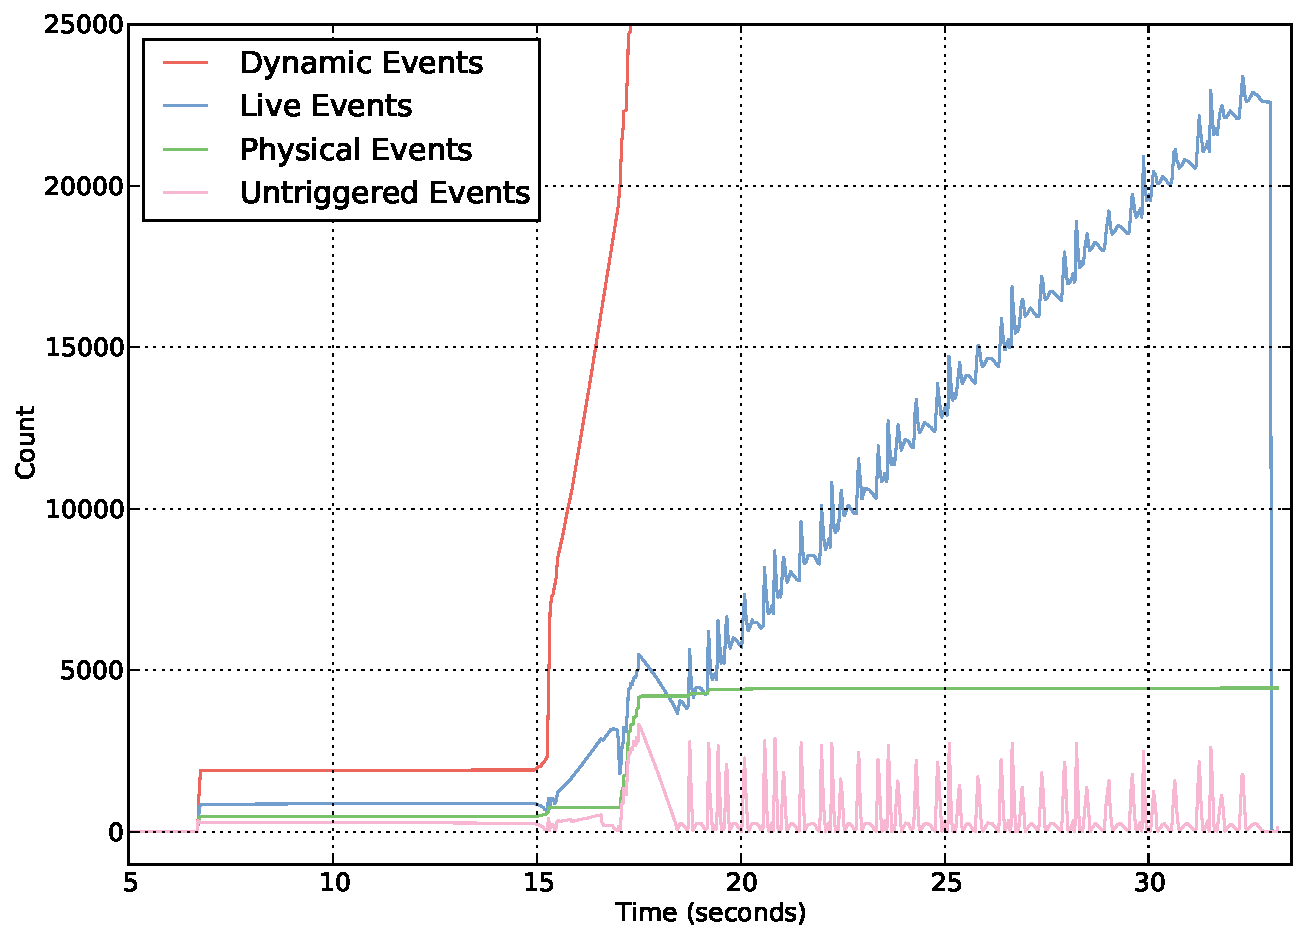
\includegraphics[scale=0.33]{figs/event_lifetimes.pdf}
\end{center}
\vspace{-6mm}
\caption{Event Liftimes - Fluid Application.\label{fig:eventlife}}
\vspace{-4mm}
\end{figure}

Figure~\ref{fig:eventlife} shows the event lifetimes in a run of the fluid application.  The total number
of events created during the application is over 260,000.

\subsection{Lock Migration}
\label{subsec:lockmig}

\subsection{Reduction Case Study}
\label{subsec:reduccase}

\subsection{Bulk-Synchronous Comparison}
\label{subsec:bulkcomp}

